\newpage
\section{Systematic tests \& Benchmark}

\subsection{Unit Testing}
To ensure that each individual component of the program works as intended, systematic unit testing was required. This was done by Whitebox \cite{testing/whiteboxtesting} testing using our knowledge of the program to create tests with Junit tests, asserting that each specific action of the module gave the expected result. Thereby ensuring that every component inside of the class works as intended and thereby having the ability to rule it out during the debugging process of a component.
\subsubsection{Jacoco}
Jacoco was a tool used by us to determine the fulfillments of our tests made to the class. From Jacoco we extracted reports on what was tested, to what degree and what needed. Helping us determine if the testing had been done thoroughly enough.\\
For the overall test coverage, we received 45 \%, which to an extent can be seen as less than adequate. But most of the uncovered programs are from the controller and the drawing map, which were difficult to test, because of how these classes were dependent on the main application class.
Instead the resources were spent on testing various utility classes and the XMLReader with an osm file for testing.\par
The most tested classes are also amongst the most central. The TagWayBuilder is responsible for building all TagWay classes. Same for the TagAddressBuilder with TagAddresses. The XMLReader reads the osm file and translates data to tags.
The model stores all tags and is responsible for Trie and the KDTree. And the Tag superclass to all the different tags is also almost completely covered.

\begin{figure}[ht]%
  \centering
  \subfloat[\centering Total Test coverage in Minion Map]{{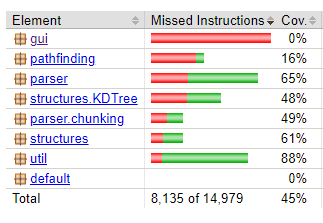
\includegraphics[width=6.25cm]{docs/material/Jacoco_Tests.png} }}\label{jacocoTestcovarage}%
  \subfloat[\centering Most test covered classes in Minion Map]{{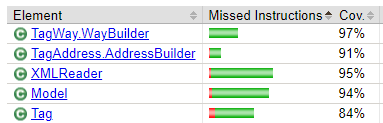
\includegraphics[width=9cm]{docs/material/Jacoco_TestResults.png}} 
    } \label{jacocoTestcovarageresult}}%
\end{figure}

\subsubsection{Improvements}
Getting more coverage, by being able to test the main application would certainly be preferred. This could be done more easily if the various classes such as drawingmap had a default constructor that could be called without the need of starting main. Another thing would be to make more of the methods static so that the tests would not need to initialize a DrawingMap to a field, and instead use the one constructed in the mapView.

\subsubsection{Un-synced Tests}
Before incorporation synchronization for the tests, there were alot of issues getting them all to parse at once in one round which was required by jacoco to file the report. This was probably caused by improper Garbage collection after each and every one of them. The tests passes individually.
Which is why you see SOME/ALL? of them being synchronized in the program. 

\subsection{Benchmarks for general operations}


The following benchmarks are performed on a pc with intel-i7 6700 processor and 16 GB 3200 MHz ram with an SSD.
\begin{table}[h]
\centering
 \begin{tabular}{ c|c }
\textbf{Operations} & \textbf{Time} \\
\hline
Drawing (through panning or zooming) & $2 \;-\; 40$ ms \\
Loading zipped file & $\sim4500$ ms \\
Pathfinding A* & $\leq 1124$ ms \\
\end{tabular}
 \caption{\centering Table for operations over Bornholm}
\end{table}

Although the drawing method seems effective compared to other general operations, it has to be run for every frame when panning. Which means that for 40 ms, the program would run at 25 frames per second.  Loading is only called once a map is chosen in the LobbyView. For a Zipped version of Bornholm, 4.5 seconds is up to our standards as it takes additional time to unzip the map. For a larger map it will take longer to load, but as the cost of loading a map only happens once on startup and not every frame loaded, the cost is not detrimental to our program.

 \subsection{Benchmarks of pathfinding}

 The following benchmarks are performed on a pc with AMD Ryzen 7 5800H processor and 16 GB 3200 MHz ram. 
 \begin{table}[h]
\centering
 \begin{tabular}{ c|c|c|c|c }
\textbf{Route} & \textbf{Dijkstra} & \textbf{A-Star} & \textbf{Gain} & \textbf{Gain percentage} \\
\hline
   Bagergade 2, 3700 Rønne to
 & 832ms & 101ms & -731s & $\sim87.9$\% \\
Nexø Busstation, 3730 Nexø
 &  &  &  &  \\
   All of the edges scanned through & 10962 edges & 2131 edges & -8.831 edges & $\sim80.6$\%  \\
\end{tabular}
 \caption{\centering Table for operations over Bornholm}
\end{table}

As we can see in the table above, the performance gains from using A-Star instead of only Dijkstra are quite substantial. It takes 87,9\% less time to calculate the shortest route. The routes found from both techniques, in this example, are exactly the same and therefore there is no loss in accuracy. But it can vary from route to route.



